%rubber: module pdflatex

\documentclass[11pt,a4paper]{article}

\usepackage[sans]{tcc_doc} % SDP style file
\usepackage[english]{babel}
\usepackage{amssymb,amsmath} % for the math symbols
\usepackage{mdwlist}
\usepackage{geometry}
\usepackage{marginnote}
\usepackage{datetime}
\usepackage{graphicx}
\usepackage{verbatim}
\usepackage{mathtools}
\usepackage{hhtensor}
\graphicspath{ {images/} }

\usepackage[boxruled,linesnumbered]{algorithm2e}
\usepackage{fmtcount}


% TODO:
% 1. Check if all new symbols have been explained when used for the first
% time.
% 2. Check if all symbols are actually being used.
% 3. Check the symbol definitions: rates, numbers, etc. to use the same main letter
% 4. Is there a way to use proper referencing of applicable and reference
% documents?



%%%%%%%%% START OF USER SETTINGS %%%%%%%%%%%%%%%%%%

% Enter here some information needed to fill in the template Title to appear
% on the front pages (will be filled in via the \sdpfrontpage command)
\newcommand{\bigdoctitle}{Implementation of the Rau-Cornwell MSMFS algorithm \xspace}
% Title to go in the "Document Status Sheet" Document number
\newcommand{\docnr}{TCC-SDP-151123-2\xspace}
% Context
\newcommand{\context}{(SDP.PIP)}
% Revision
\newcommand{\revision}{2\xspace}
% Author(s)
\newcommand{\docauthor}{T.J.\ Cornwell\xspace}
% Lead author (goes in the footer)
\newcommand{\leadauthor}{T.J.\ Cornwell\xspace}
% Release date (YYYY-MM-DD)
\newcommand{\docudate}{\today\ \currenttime}
% Document classification
\newcommand{\classification}{Unrestricted}
% Status of the document (draft/final/etc.)
\newcommand{\docstatus}{Draft\xspace}

% The definitions below are used for the signature tables in the preamble of
% the document
\newcommand{\firstsigname}{Name 1 - to be filled in}
\newcommand{\firstsigdesignation}{Designation 1 - to be filled in}
\newcommand{\firstsigaffiliation}{Affiliation 1 - to be filled in}

\newcommand{\secondsigname}{Name 2 - to be filled in}
\newcommand{\secondsigdesignation}{Designation 2 - to be filled in}
\newcommand{\secondsigaffiliation}{Affiliation 2 - to be filled in}

% Table with version numbers
\newcommand{\versiontable}{
  \begin{tabularx}{\textwidth}{|X|X|X|X|}
    \hline
    \bf{Version} & {\bf Date of issue} & {\bf Prepared by} & {\bf Comments}\\
    \hline
  \end{tabularx}
}

%%%%%%%%%%%%% END OF USER SETTINGS %%%%%%%%%%%%%%%%%%%

% Table with signatures
\newcommand{\signaturetable}[3]{
  \begin{tabularx}{\textwidth}{|X|X|X|}
    \hline
    Name & Designation & Affilitation\\
    \hline
    {#1} & {#2} & {#3}\\
    \hline
    Signature \& Date: & & \\
    & & \\
    & & \\
    \hline
  \end{tabularx}
}



% Table with affiliations
\newcommand{\organisationtable}{
  \begin{center}
    \sffamily{\bf ORGANISATION DETAILS}\end{center}
  \begin{table}[htb]
    \centering
    \begin{tabular}[htb]{|l|l|}
      \hline
      Name & Science Data Processor Consortium\\
      \hline
    \end{tabular}
  \end{table}
}


%%%%%%%%%%%%%%%%%%%% START YOUR DOCUMENT HERE %%%%%%%%%%%%%%%%%

\newcommand{\subsubsubsection}[1]{\noindent{\bf{#1}}}

%%%% Please DO USE the symbol definitions listed below to preserve
%%%% consistency.

%%%% If you need a new symbol, please add it here. If really want to modify
%%%% one, do so, just take care to do a search-and-replace for the entire document
% Symbol definitions
\newcommand{\bytes}{b} % Length of a complex number in bytes
\newcommand{\cbytes}{b} % Length of a real number in bytes
\newcommand{\rbytes}{b} % Length of a complex number in bytes
\newcommand{\bl}{B} % Baseline length
\newcommand{\maxbl}{B_{\mathrm{max}}} % Maximum baseline length
\newcommand{\membw}{B_\mathrm{mem}} % Memory bandwidth
\newcommand{\pciebw}{B_\mathrm{PCIe}} % PCI-e bandwidth
\newcommand{\viscompr}{C} % Compression factor of visibilities for gridding
                          % for facets
\newcommand{\vism}{\mathbb{D}} % Matrix of observed visibilities
\newcommand{\da}{D_{\mathrm A}} % Extent of aperture
\newcommand{\ds}{D_{\mathrm s}} % Diameter of antennas/stations
\newcommand{\reff}{f_\mathrm{ref}} % Reference frequency
\newcommand{\fcc}{F_{\mathrm{cc}}} % Convolution kernel computational cost
\newcommand{\fci}{F_{\mathrm{ci}}} % Factor between bandwidth and FLOPS (bytes/ops)
\newcommand{\fgrid}{F_{\mathrm{grid}}} % Gridding cost
\newcommand{\fpatch}{f_\mathrm{patch}} % Fraction of the maximum baseline below which the uv coverage is almost filled
\newcommand{\fpr}{F_\mathrm{pr}} % Cost for phase rotation
\newcommand{\gainm}{\mathbb{G}} % 2x2 block diagonal matrix of complex gains
% To change to N_something
\newcommand{\modskyvism}{\mathbb{M}} % Matrix of model sky visibilities
\newcommand{\skymodbufsize}{M_\mathrm{buf,skymod}} % Size of the sky model buffer
\newcommand{\visbufsize}{M_\mathrm{buf,vis}} % Size of the visibility buffer
\newcommand{\visbufsizespec}{M^\mathrm{spec}_\mathrm{buf,vis}} % Size of the visibility buffer needed for spectral line processing
\newcommand{\visbufsizecont}{M^\mathrm{cont}_\mathrm{buf,vis}} % Size of the visibility buffer needed for continuum imaging
\newcommand{\bufsize}{M_\mathrm{cu,buf}} % Size of buffer
\newcommand{\slowmemsize}{M_\mathrm{cu,pool}} %	Size of slow working memory
\newcommand{\cumemsize}{M_\mathrm{cu,work}} % Size of working memory of compute unit
\newcommand{\imgsize}{M_\mathrm{image}} % Size of image (bytes)
\newcommand{\imgsizeoneax}{M_\mathrm{image,ax}}	% Image size along one axis
\newcommand{\nbyteperpix}{N_\mathrm{byte,pix}} % Number of bytes per pixel
%\newcommand{\nbytepervis}{N_\mathrm{byte,vis}} % Number of bytes per pixel
\newcommand{\targgridsize}{M_\mathrm{target}} %	Target grid size (per facet)
\newcommand{\uvgridsize}{M_{uv,\mathrm{grid}}} % Size of the uv-grid (bytes)
\newcommand{\vissize}{M_\mathrm{vis}} % Size of visibility data (bytes)
\newcommand{\wgridsize}{M_\mathrm{weight\_grid}} % Size of weight grid (bytes)
\newcommand{\gridcachesize}{M_{w,\mathrm{cache}}} % Cache size of
                                % gridding kernel
\newcommand{\ntel}{N_\mathrm{a}} % Number of antennas or stations in the array
\newcommand{\nateam}{N_\mathrm{A}} % Number of A-team sources
\newcommand{\ngridpakern}{N_\mathrm{AA}} % Number of grid points for A-kernel support (along one axis)
\newcommand{\naccvis}{N_\mathrm{apv}} % Number of accesses per visibility
\newcommand{\navg}{N_\mathrm{avg}} % Number of averages
\newcommand{\nbins}{N_\mathrm{bin}} % Number of bins
\newcommand{\nbeam}{N_\mathrm{beam}} % Number of beams simultaneously observed by the array
\newcommand{\rma}{N_{rma}} % Number of flops in real multiply and add
\newcommand{\cma}{N_{cma}} % Number of flops in complex multiply and add
\newcommand{\nbits}{N_\mathrm{bit}} %	Number of bits
\newcommand{\nbl}{N_\mathrm{bl}} % Number of baselines
\newcommand{\nbyteacc}{N_\mathrm{bpa}} % Number of bytes per access
\newcommand{\nbyte}{N_\mathrm{byte}} % Number of bytes
\newcommand{\nch}{N_\mathrm{ch}XXXWANT TO USE NF HERE} % Number of channels
\newcommand{\ncompu}{N_\mathrm{cu}} % Number of compute units
\newcommand{\ndatait}{N_\mathrm{datait}} % Number of data items required per source (e.g. postion)
\newcommand{\ngridp}{N_\mathrm{cvff}} % Number of grid points along one axis for the gridding convolution function
\newcommand{\nfch}{N_\mathrm{f}} % Number of frequency channels
\newcommand{\nfchcorr}{N_\mathrm{f,corr}} % Number of frequency channels output by the correlator
\newcommand{\nfnosmear}{N_\mathrm{f,smear}} % Number of frequency channels set by smearing limit
\newcommand{\nfchgrid}{N_\mathrm{f,grid}} % Number of frequency channels to be gridded
\newcommand{\nfchdegrid}{N_\mathrm{f,de-grid}} % Number of frequency channels to be de-gridded
\newcommand{\nfchout}{N_\mathrm{f,out}} % Number of output frequency channels
                                % (to be FFT-ed and reprojected or output from
                                % the CSP pulsar timing backend
\newcommand{\nfchdist}{N_\mathrm{f,distribute}} % Minimum number of frequencies needed to maintain distributability
\newcommand{\nfkernel}{N_\mathrm{f,kernel}} %Number of convolution kernels needed to cover frequency axis for a particular baseline
\newcommand{\nfacet}{N_\mathrm{facet}} % Number of facets along one axis
\newcommand{\facetoverlap}{r_\mathrm{facet}} %Facet overlap overhead
\newcommand{\nflop}{N_\mathrm{FLOP}} % Number of floating point operations
\newcommand{\nflopsamp}{N_\mathrm{FLOPsamp}} % Number of floating point
                                % operations per sample
\newcommand{\nflopvis}{N_\mathrm{FLOPvis}} % Number of floating point
                                % operations per visibility 
\newcommand{\npixgrid}{N_\mathrm{grid}} % Number of pixels in the grid (i.e. the square of the linear dimension)
\newcommand{\ngridwkern}{N_\mathrm{GW}} % Number of grid points for w-kernel
                                % support (along one axis)
\newcommand{\nit}{N_\mathrm{it}} % Number of iterations
\newcommand{\nawkern}{N_\mathrm{kernel}} % Linear size of combined A and w-kernels
\newcommand{\nmaj}{N_\mathrm{major}} % Number of major CLEAN cycles
\newcommand{\nmin}{N_\mathrm{minor}} % Number of minor CLEAN cycles
\newcommand{\nselfcal}{N_\mathrm{SelfCal}} %Number of self cal loops
% TODO: Factors should have another letter than N
\newcommand{\facgridoffdiagmuller}{N_\mathrm{mm}} % Factor to account for
                                % gridding of off-diagonal Mueller terms
% TODO: Factors should have another letter than N
\newcommand{\nops}{N_\mathrm{ops}} % Number of operations
\newcommand{\npatchpix}{N_\mathrm{patch,pix}} % Number of pixels of PSF to be used in minor cycle decorrelation
\newcommand{\npix}{N_\mathrm{pix}} % Number of pixels along one axis of a grid
\newcommand{\npixfacet}{N_\mathrm{pix,facet}} % Number of pixels along one axis of a single image facet
\newcommand{\npol}{N_\mathrm{pol}} % Number of polarisation products
\newcommand{\nsubint}{N_\mathrm{subint}} % Number of sub-integrations
\newcommand{\ntslot}{N_t} % Number of time slots
\newcommand{\ntaylor}{N_\mathrm{Tt}} % Number of Taylor terms
\newcommand{\ntslotave}{N_{t,\mathrm{av}}} % Number of time slots that are averaged (in de-mixing)
\newcommand{\nvis}{N_\mathrm{vis}} % Number of visibilities
\newcommand{\nvisrate}{R_{vis}} % Number of visibilities per second\\
% TODO: what kind of qfac?
\newcommand{\qfacbw}{Q_\mathrm{bw}} % Quality factor
\newcommand{\qfacreuse}{Q_\mathrm{fcv}} % Factor to allow for the reuse of functions between neighbouring frequency channels
\newcommand{\qfacfov}{Q_\mathrm{FoV}} % Quality factor defining how much bigger the diameter of the field of view is than the first zero of the Airy function
\newcommand{\facgridovers}{Q_\mathrm{GCF}} % Gridding oversampling factor
\newcommand{\facmsmf}{Q_\mathrm{MSMF}} % Factor to account for multiple subtractions (multi-frequency multi-scale CLEAN)
\newcommand{\qfacbeamovers}{Q_\mathrm{pix}} % Quality factor defining the
                                % oversampling of the synthesised beam
% TODO: what kind of qfac?
\newcommand{\qfac}{Q_t} % Quality factor
\newcommand{\corrfacw}{Q_w} % Correction factor for w values (0 to 1)
\newcommand{\earthrad}{R_\mathrm{Earth}} % Radius of the Earth ($6400\times 10^3$\,m)
\newcommand{\comprate}{R} % Compute rate (FLOPS)
\newcommand{\compratespec}{R^\mathrm{spec}} % Compute rate for spectral line processing
\newcommand{\compratecont}{R^\mathrm{cont}} % Compute rate for continuum imaging
\newcommand{\compratefast}{R^\mathrm{fast}} % Compute rate for fast imaging
\newcommand{\covm}{\mathbb{R}} % Covariance matrix
\newcommand{\covmfilt}{\mathbb{R}_\mathrm{filt}} % Filtered covariance matrix
\newcommand{\bwtoworkmem}{R_\mathrm{bw,mem}} % Bandwidth to working memory
\newcommand{\maxmembw}{R_\mathrm{bw,max}} % Maximum memory bandwidth of
                                % compute unit
\newcommand{\convkernflops}{R_\mathrm{CCF}} % Convolution kernel compute rate (FLOPS)
\newcommand{\fftflops}{R_\mathrm{FFT}} % FFT compute rate (FLOPS)
\newcommand{\flagflops}{R_\mathrm{flag}} % FLOP rate to do flagging on input visibilities
\newcommand{\griddingflops}{R_\mathrm{grid}} % Gridding compute rate (FLOPS)
\newcommand{\phaserotflops}{R_\mathrm{PR}} % Phase rotation compute rate (FLOPS)
\newcommand{\reprojflops}{R_\mathrm{RP}} % Re-projection compute rate (FLOPS)
\newcommand{\rcorr}{R_\mathrm{s}} % Correlator output rate (samples/sec)
\newcommand{\peakflop}{R_\mathrm{peak}} % Peak FLOPS of compute unit
% TODO - verschil met max mem bw of compute unit?
% TODO - verschil memory bw and bw to buffer?
\newcommand{\IO}{{R_\mathrm{IO}}} %IO rate
\newcommand{\maxiobwbuff}{R_\mathrm{bw,I/O,max}} % Maximum I/O bandwidth of compute unit to buffer
\newcommand{\bwbuff}{R_\mathrm{bw,I/O}} % Bandwidth to buffer
\newcommand{\bwbuffcont}{R^\mathrm{cont}_\mathrm{bw,I/O}} % Bandwidth to
                                % buffer for cotinuum imaging
\newcommand{\bwbuffspec}{R^\mathrm{spec}_\mathrm{bw,I/O}} % Bandwidth to
                                % buffer for spectral line processing
\newcommand{\nsource}{N_\mathrm{source}} % Number of sources
\newcommand{\telsensit}{S} % Telescope sensitivity
\newcommand{\corrdumpt}{t_\mathrm{dump}} % Correlator dump time (sec)
\newcommand{\compt}{t_{\mathrm{comp}}} % Computation time
\newcommand{\gridkernupdate}{t_\mathrm{kernel,update}} % Update timescale for gridding kernel
\newcommand{\lsmupdate}{t_\mathrm{LSM}} % Update timescale for the LSM
\newcommand{\obst}{t_{\mathrm{obs}}} % Observation time
\newcommand{\snapshot}{t_\mathrm{snap}} % Snapshot duration
\newcommand{\minsnapshot}{t_\mathrm{snap,min}} % Minimum duration of a snapshot in which w-correction is not dominated by Earth's curvature
\newcommand{\optsnapshot}{t_\mathrm{snap,opt}} % Optimum snapshot duration (sec)
\newcommand{\subint}{t_\mathrm{subint}} % Subintegration time
\newcommand{\uv}{uv} % Visibility coordinates
\newcommand{\uvw}{u,v,w} % Visibility coordinates
\newcommand{\w}{w} % Visibility w coordinate
\newcommand{\nbytepervis}{N_\mathrm{byte,vis}} %Memory per individual visibility 
\newcommand{\maxwdev}{\Delta w_\mathrm{max}} % Maximum deviation of the w
                                % coordinate due to the Earth's curvature
\newcommand{\minwdev}{\Delta w_\mathrm{min}} % Minimum deviation of the w
                                % coordinate due to the Earth's curvature
\newcommand{\spfiltm}{\mathbb{W}_\mathrm{filt}} % Spatial filter matrix
\newcommand{\fres}{\Delta f} % Frequency resolution
\newcommand{\tressmear}{t_\mathrm{smear}} % Smearing Time resolution (sec)
\newcommand{\tres}{t_{res}} % Time resolution (sec)
\newcommand{\fracconvfuncamp}{\epsilon_\omega} % Fraction of maximal amplitude of envelope of convolution function
\newcommand{\compeff}{\eta_\mathrm{comp}} % Computational efficiency
\newcommand{\fracfband}{\eta_f} % Fraction of frequency band
\newcommand{\beamsq}{\theta_\mathrm{bs}} % Beam squint
\newcommand{\fovdiam}{\theta_\mathrm{FoV}} % Angular diameter of the field of view (rad)
\newcommand{\pixres}{\theta_\mathrm{pix}} % Angular resolution of pixel size (rad)
\newcommand{\beamdiam}{\theta_\mathrm{PSF}} % Angular diameter of the synthesised beam (rad)
\newcommand{\wavel}{\lambda} % Wavelength
\newcommand{\maxwavel}{\lambda_\mathrm{max}} % Maximum wavelength
\newcommand{\minwavel}{\lambda_\mathrm{min}} % Minimum wavelength
\newcommand{\maxwavelsubb}{\lambda_{\mathrm{sub,max}}} % Maximum wavelength of an imaging sub-band (channels over which image and pixel size are matched)
\newcommand{\minwavelsubb}{\lambda_\mathrm{sub,min}} % Minimum wavelength of an imaging sub-band (channels over which image and pixel size are matched)
\newcommand{\earthrot}{\Omega_\mathrm{E}} % Angular velocity of the Earth (7.27 10-5 rad/sec)
\newcommand{\epsilonf}{\epsilon_f}  %Fraction of a uv cell that we allow uv track to move in time- or frequency- smearing-limited averaging
% Other command definitions
\newcommand{\Qkernel}{Q_\mathrm{kernel}} %Convolution kernel quality factor, for kernel re-use in frequency
\newcommand{\bs}{\texttt{\char`\\}}



\begin{document}

% load automatic pages
\tccfrontpage

\sdptableofcontents

% Add here the abbreviations used in your document
\sdplistofabbreviations
\begin{basedescript}{\desclabelstyle{\pushlabel}\desclabelwidth{6em}}
    \item[CDR] Critical Design Review \vspace{-0.2cm}
    \item[CPU] Central Processing Unit\vspace{-0.2cm}
    \item[CSP] Central Signal Processor\vspace{-0.2cm}
    \item[CUFFT] \textcolor{red}{Define it.}\vspace{-0.2cm}
    \item[DFT] \textcolor{red}{Only used once, in a title. Remove/expand?}\vspace{-0.2cm}
    \item[DM] \textcolor{red}{Define it.}\vspace{-0.2cm}
    \item[EoR] Epoch of Reionisation\vspace{-0.2cm}
    \item[FFT] Fast Fourier Transform\vspace{-0.2cm}
    \item[FLOP] Floating Point Operations \vspace{-0.2cm}
    \item[FLOPS] Floating Point Operations per Second \vspace{-0.2cm}
    \item[FoV] Field of View\vspace{-0.2cm}
    \item[GPU] Graphics Processing Unit \vspace{-0.2cm}
    \item[ICD] Interface Control Document\vspace{-0.2cm}
    \item[LMA] Levenberg-Marquardt Algorithm \vspace{-0.2cm}
    \item[LOFAR] LOw Frequency ARray\vspace{-0.2cm}
    \item[LSM] Local Sky Model\vspace{-0.2cm}
    \item[MS-MFS] Multi-Scale Multi-Frequency Synthesis\vspace{-0.2cm}
    \item[NVRAM] \textcolor{red}{Define it.} \vspace{-0.2cm}
    \item[OCLD] Optimised Candidate List and Data \vspace{-0.2cm}
    \item[PDR] Preliminary Design Review\vspace{-0.2cm}
    \item[RFI] Radio Frequency Interference\vspace{-0.2cm}
    \item[PSF] \textcolor{red}{Define it.} \vspace{-0.2cm}
    \item[PSS] Pulsar Search\vspace{-0.2cm}
    \item[PST] Pulsar Timing\vspace{-0.2cm}
    \item[SDP] Scientific Data Processor\vspace{-0.2cm}
    \item[SKA] Square Kilometre Array\vspace{-0.2cm}
    \item[SKAO] SKA Organisation\vspace{-0.2cm}
    \item[WCS] \textcolor{red}{Define it.} \vspace{-0.2cm}
%    \item[] \vspace{-0.2cm}
\end{basedescript} 

\newcommand{\nuno}{{\left(\frac{\nu}{\nu_0}\right)}}
\newcommand{\dnuno}{{\left(\frac{\nu-\nu_0}{\nu_0}\right)}}

\newcommand{\dg}{^\dag}
\newcommand{\X}{\vec{x}}
\newcommand{\Xd}{\vec{{x}^\dag}}
\newcommand{\B}{\vec{b}}
\newcommand{\Bd}{\vec{b^\dag}}
\newcommand{\A}{{\tens{A}}}
\newcommand{\Ad}{{\tens{A^\dag}}}
\newcommand{\F}{{\tens{F}}}
\newcommand{\Fd}{{\tens{F^\dag}}}
\newcommand{\He}{{\tens{H}}}
\newcommand{\Sa}{{\tens{S}}}
\newcommand{\Sd}{{\tens{S^\dag}}}
\newcommand{\Sna}{\tens{{S_{\nu}}}}
\newcommand{\Snd}{\tens{{S_{\nu}^\dag}}}
\newcommand{\T}{{\tens{T}}}
\newcommand{\W}{{\tens{W}}}
\newcommand{\Wd}{{\tens{W^\dag}}}
\newcommand{\Pb}{{P_b}}

\newcommand{\Wim}{{\tens{W^{im}}}}
\newcommand{\Wimd}{{\tens{{W^{im}}^\dag}}}
\newcommand{\Wnt}{{\tens{W^{mfs}_t}}}
\newcommand{\Wntd}{{\tens{{W^{mfs}_t}^\dag}}}
\newcommand{\Wnp}{{\tens{W^{mfs}_p}}}
\newcommand{\Wnpd}{{\tens{{W^{mfs}_p}^\dag}}}
\newcommand{\Wnq}{{\tens{W^{mfs}_q}}}
\newcommand{\Wnqd}{{\tens{{W^{mfs}_q}^\dag}}}
\newcommand{\Wimn}{{\tens{W^{im}_{\nu}}}}
\newcommand{\Wimnd}{{\tens{{W^{im}_{\nu}}^\dag}}}

\newcommand{\wnt}{{w_{\nu}^t}}
\newcommand{\wnq}{{w_{\nu}^q}}
\newcommand{\wntq}{{w_{\nu}^{t+q}}}
\newcommand{\Wntn}{{\tens{w^{mfs}_{t,\nu}}}}
\newcommand{\Wntnd}{{\tens{{w^{mfs}_{t,\nu}}^\dag}}}
\newcommand{\Wnpn}{{\tens{W^{mfs}_{p,\nu}}}}
\newcommand{\Wnpnd}{{\tens{{W^{mfs}_{p,\nu}}^\dag}}}

\newcommand{\pd}{{\partial}}
\newcommand{\mi}{{m_{I}}}
\newcommand{\R}{{R}}
\newcommand{\Rd}{{R^\dag}}
\newcommand{\I}{{\vec{I}}}


% Add here the symbols used in your document
\clearpage \sdplistofsymbols
\begin{basedescript}{\desclabelstyle{\pushlabel}\desclabelwidth{6em}}
\item[$\bytes$] Length of a complex number in bytes \vspace{-0.2cm}
\item[$\cbytes$] Length of a complex number in bytes \vspace{-0.2cm}
\item[$\rbytes$] Length of a real number in bytes \vspace{-0.2cm}
\item[$\bl$] Baseline length / GPU memory bandwidth \vspace{-0.2cm}
\item[$\maxbl$] Maximum baseline length \vspace{-0.2cm}
\item[$\membw$] Memory bandwidth \vspace{-0.2cm}
\item [$\pciebw$] PCI-e bandwidth \vspace{-0.2cm}
\item[$\viscompr$] Compression factor of visibilities for grdding for facets
  \textcolor{red}{This symbol is not used in the document, consider removing.}
  \vspace{-0.2cm}
\item[$\vism$] Matrix of observed visibilities \vspace{-0.2cm}
\item[$\da$] Extent of aperture \vspace{-0.2cm}
\item[$\ds$] Diameter of antennas/stations \vspace{-0.2cm}
\item[$\reff$] Reference frequency\vspace{-0.2cm}
\item[$\fcc$] Convolution kernel computational cost\vspace{-0.2cm}
\item[$\fci$] Factor between bandwidth and FLOPS (bytes/operations)\vspace{-0.2cm}
\item[$\fgrid$] Gridding cost\vspace{-0.2cm}
\item[$\fpatch$] Fraction of the maximum baseline below which the $\uv$
  coverage is almost filled\vspace{-0.2cm}
\item[$\fpr$] Cost for phase rotation\vspace{-0.2cm}
\item[$\gainm$] 2$\times$2 block diagonal matrix of complex
  gains\vspace{-0.2cm}
\item[$\modskyvism$] Matrix of model sky visibilities\vspace{-0.2cm}
\item[$\skymodbufsize$] Size of the sky model buffer\vspace{-0.2cm}
\item[$\visbufsize$] Size of the visibility buffer \vspace{-0.2cm}
\item[$\visbufsizespec$] Size of the visibility buffer needed for spectral line processing\vspace{-0.2cm}
\item[$\visbufsizecont$] Size of the visibility buffer needed for continuum imaging\vspace{-0.2cm}
\item[$\bufsize$] Size of buffer \vspace{-0.2cm}
\item[$\slowmemsize$] Size of slow working memory \vspace{-0.2cm}
\item[$\cumemsize$] Size of working memory of compute unit \vspace{-0.2cm}
\item[$\imgsize$] Size of image (bytes) \vspace{-0.2cm}
\item[$\imgsizeoneax$] Image size along one axis \vspace{-0.2cm}
\item[$\targgridsize$] Target grid size (per facet) \vspace{-0.2cm}
\item[$\uvgridsize$] Size of the $\uv$ grid (bytes) \vspace{-0.2cm}
\item[$\vissize$] Size of visibility data (bytes) \vspace{-0.2cm}
\item[$\wgridsize$] Size of weight grid (bytes)\vspace{-0.2cm}
\item[$\gridcachesize$] Cache size of gridding kernel \vspace{-0.2cm}
\item[$\nbins$] Number of bins \vspace{-0.2cm}
\item[$\ntel$] Number of antennas or stations in the array
  \vspace{-0.2cm}
\item[$\nateam$] Number of A-team sources \vspace{-0.2cm}
\item[$\ngridpakern$] Number of grid points for A-kernel support (along one
  axis) \vspace{-0.2cm}
\item[$\naccvis$] Number of accesses per visibility \vspace{-0.2cm}
\item[$\navg$] Number of averages\vspace{-0.2cm}
\item[$\nbeam$] Number of beams simultaneously observed by the array
  \vspace{-0.2cm}
\item[$\nbits$] Number of bits\vspace{-0.2cm}
\item[$\rma$] Number of flops in real multiply and add\vspace{-0.2cm}
\item[$\cma$] Number of flops in complex multiply and add\vspace{-0.2cm}
\item[$\nbl$] Number of baselines \vspace{-0.2cm}
\item[$\nbyteacc$] Number of bytes per access \vspace{-0.2cm}
\item[$\nbyte$] Number of bytes \vspace{-0.2cm}
\item[$\nbyteperpix$] Number of bytes per pixel \vspace{-0.2cm}
\item[$\nbytepervis$] Number of bytes per individual visibility 

\item[$\nch$] Number of channels \vspace{-0.2cm}
\item[$\ncompu$] Number of compute units \vspace{-0.2cm}
\item[$\ndatait$] Number of data items required per source (e.g. position)\vspace{-0.2cm}
\item[$\ngridp$] Number of grid points along one axis for the gridding
  convolution function \vspace{-0.2cm}
\item[$\nfch$] Number of frequency channels/sub-bands \vspace{-0.2cm}
\item[$\nfchcorr$] Number of frequency channels output by the correlator
  \vspace{-0.2cm}
\item[$\nfchgrid$] Number of frequency channels to be gridded
  \vspace{-0.2cm}
\item[$\nfchdegrid$] Number of frequency channels to be de-gridded
  \vspace{-0.2cm}
\item[$\nfchout$] Number of frequency channels to be FFT-ed and reprojected
  (output) or output from the CSP pulsar timing backend\vspace{-0.2cm}
\item[$\nfchdist$] Minimum number of frequency channels to maintain distributability in the SDP
\item[$\nfkernel$] Number of convolution kernels needed to cover frequency axis for a given baseline
\item[$\nfacet$] Number of facets along one axis \vspace{-0.2cm}
\item[$\nflop$] Number of floating point operations
  \vspace{-0.2cm}
\item[$\nflopsamp$] Number of floating point operations per sample
  \vspace{-0.2cm}
\item[$\nflopvis$] Number of floating point operations per visibility
\item[$\npixgrid$] Number of pixels in the grid (i.e. the square of the linear
  dimension) \vspace{-0.2cm}
\item[$\ngridwkern$] Number of grid points for w-kernel support (along one
  axis) \vspace{-0.2cm}
\item[$\nit$] Number of iterations \vspace{-0.2cm}
\item[$\nawkern$] Linear size of combined A and $\w$-kernels \vspace{-0.2cm}
\item[$\nmaj$] Number of major CLEAN cycles (within each self-cal loop if appropriate) \vspace{-0.2cm}
\item[$\nselfcal$] Number of self-calibration cycles \vspace{-0.2cm}
\item[$\nmin$] Number of minor CLEAN cycles (within each major cycle loop if appropriate)\vspace{-0.2cm}
\item[$\facgridoffdiagmuller$] Factor to account for gridding of off-diagonal
  M\"uller terms \vspace{-0.2cm}
\item[$\nops$] Number of operations \vspace{-0.2cm}
\item[$\npatchpix$] Number of pixels of PSF to be used in minor cycle
  decorrelation \vspace{-0.2cm}
\item[$\npix$] Number of pixels along one axis of a grid\vspace{-0.2cm}
\item[$\npixfacet$] Number of pixels on one side of a facet \vspace{-0.2cm}
\item[$\npol$] Number of polarisation products \vspace{-0.2cm}
\item[$\nsource$] Number of sources \vspace{-0.2cm}
\item[$\ntslot$] Number of time slots \vspace{-0.2cm}
\item[$\ntaylor$] Number of Taylor terms (in MS-MFS)\vspace{-0.2cm}
\item[$\ntslotave$] Number of time slots that are averaged (in de-mixing)
  \vspace{-0.2cm}
\item[$\nvis$] Number of visibilities in an observation \vspace{-0.2cm}
\item[$\qfacbw$] Quality factor \vspace{-0.2cm}
\item[$\qfacreuse$] Factor to allow for the reuse of functions between
  neighbouring frequency channels \vspace{-0.2cm}
\item[$\qfacfov$] Quality factor defining how much bigger the diameter of the
  field of view is than the first zero of the Airy function \vspace{-0.2cm}
\item[$\facgridovers$] Gridding oversampling factor \vspace{-0.2cm}
\item[$\facmsmf$] Factor to account for multiple subtractions (multi-frequency
  multi-scale CLEAN\vspace{-0.2cm}
\item[$\qfacbeamovers$] Quality factor defining the oversampling of the
  synthesised beam \vspace{-0.2cm}
\item[$\qfac$] Quality factor \vspace{-0.2cm}
\item[$\Qkernel$] Convolution kernel quality factor, for kernel re-use in frequency
\item[$\corrfacw$] Correction factor for w values (0 to 1) \vspace{-0.2cm}
\item[$\earthrad$] Radius of the Earth ($6400\times 10^3$\,m) \vspace{-0.2cm}
\item[$\covm$] Covariance matrix \vspace{-0.2cm}
\item[$\covmfilt$] Filtered covariance matrix \vspace{-0.2cm}
\item[$\comprate$] Compute rate (FLOPS) \vspace{-0.2cm}
\item[$\compratespec$] Compute rate (FLOPS) for spectral line processing \vspace{-0.2cm}
\item[$\compratecont$] Compute rate (FLOPS) for continuum imaging \vspace{-0.2cm}
\item[$\compratefast$] Compute rate (FLOPS) for fast imaging \vspace{-0.2cm}
\item[$\bwtoworkmem$] Bandwidth to working memory \vspace{-0.2cm}
\item[$\maxmembw$] Maximum memory bandwidth of compute unit \vspace{-0.2cm}
\item[$\peakflop$] Peak FLOPS of compute unit \vspace{-0.2cm}
\item[$\maxiobwbuff$] Maximum I/O bandwidth of compute unit to buffer
  \vspace{-0.2cm}
\item[$\bwbuff$] Bandwidth to buffer \vspace{-0.2cm}
\item[$\bwbuffcont$] Bandwidth to buffer for continuum imaging\vspace{-0.2cm}
\item[$\bwbuffspec$] Bandwidth to buffer for spectral line processing\vspace{-0.2cm}
\item[$\convkernflops$] Convolution kernel compute rate (FLOPS)\vspace{-0.2cm}
\item[$\fftflops$] FFT compute rate (FLOPS)\vspace{-0.2cm}
\item[$\griddingflops$] Gridding compute rate (FLOPS)\vspace{-0.2cm}
\item[$\phaserotflops$] Phase rotation compute rate (FLOPS)\vspace{-0.2cm}
\item[$\reprojflops$] Re-projection compute rate (FLOPS)\vspace{-0.2cm}
\item[$\rcorr$] Correlator output rate\vspace{-0.2cm} TRY TO REMOVE
\item[$\facetoverlap$]  ratio for linear size increase of facets to account for overlap, typically 1.2-1.5 \vspace{-0.2cm}
\item[$\telsensit$] Telescope sensitivity \vspace{-0.2cm} TRY TO REMOVE
\item[$\corrdumpt$] Correlator dump time (sec) \vspace{-0.2cm}
\item[$\compt$] Computation time \vspace{-0.2cm}
\item[$\gridkernupdate$] Update timescale for gridding kernel \vspace{-0.2cm}
\item[$\lsmupdate$] Update timescale for the LSM \vspace{-0.2cm}
\item[$\obst$] Observation time \vspace{-0.2cm}
\item[$\snapshot$] Snapshot duration \vspace{-0.2cm}
\item[$\minsnapshot$] Minimum duration of a snapshot in which w-correction is
  not dominated by the Earth's curvature \vspace{-0.2cm}
\item[$\optsnapshot$] Optimum snapshot duration (sec) \vspace{-0.2cm}
\item[$\subint$] Sub-integration time\vspace{-0.2cm}
\item[$\uvw$] Visibility coordinates \vspace{-0.2cm}
\item [$\w$] Visibility $w$ coordinate \vspace{-0.2cm}
\item[$\maxwdev$] Maximum deviation of the $w$ coordinate due to the Earth's
  curvature \vspace{-0.2cm}
\item[$\minwdev$] Minimum deviation of the $w$ coordinate due to the Earth's
  curvature \vspace{-0.2cm}
\item[$\spfiltm$] Spatial filter matrix \vspace{-0.2cm}
\item[$\fres$] Frequency resolution \vspace{-0.2cm}
\item[$\tres$] Time resolution (sec) \vspace{-0.2cm}
\item[$\tressmear$]  Smearing Time resolution (sec)  \vspace{-0.2cm}
\item[$\fracconvfuncamp$] Fraction of maximal amplitude of envelope of
  convolution function \vspace{-0.2cm}
\item[$\compeff$] Computational efficiency \vspace{-0.2cm}
\item[$\fracfband$] Fraction of frequency band \vspace{-0.2cm}
\item[$\beamsq$] Beam squint \vspace{-0.2cm}
\item[$\fovdiam$] Angular diameter of the field of view (rad) \vspace{-0.2cm}
\item[$\pixres$] Angular resolution of pixel size (rad) \vspace{-0.2cm}
\item[$\beamdiam$] Angular diameter of the synthesised beam (rad)
  \vspace{-0.2cm}
\item[$\wavel$] Wavelength \vspace{-0.2cm}
\item[$\maxwavel$] Maximum wavelength \vspace{-0.2cm}
\item[$\minwavel$] Minimum wavelength \vspace{-0.2cm}
\item[$\maxwavelsubb$] Maximum wavelength of an imaging sub-band (channels
  over which image and pixel size are matched) \vspace{-0.2cm}
\item[$\minwavelsubb$] Minimum wavelength of an imaging sub-band (channels
  over which image and pixel size are matched) \vspace{-0.2cm}
\item[$\earthrot$] Angular velocity of the Earth
  ($7.27\times10^{-5}$\,rad/sec) \vspace{-0.2cm}
\item[$\epsilonf$] Fraction of a uv cell that we allow uv track to move in time- or frequency- smearing-limited averaging \vspace{-0.2cm}
\end{basedescript}

\sdplistoffigures

\sdplistoftables

% Add here the executive summary
\sdpsummary


\newpage

% Add to the table the list of applicable and reference documents (this is NOT
% meant for your usual bibiliography, only for SKA docs)
\sdpreferencedocs

\subsection*{Applicable Documents}

The following documents are applicable to the extent stated herein. In the
event of conflict between the contents of the applicable documents and this
document, \emph{the applicable documents} shall take precedence.

 \begin{center}{
 \begin{tabularx}{\textwidth}{|l|X|}
     \hline
     \bf{Reference} & \bf{Reference}\\
     \bf{Number} & \\
     \hline
     {\bf [AD01]} & Dewdney, P. E. (2013). SKA1 System Baseline Design. SKA Office\\
     {\bf [AD02]} & McCool, R., Cornwell, T. (2013). Miscellaneous Corrections
     to the Baseline Design\\
     {\bf [AD03]} & SKA Phase 1 System (Level 1) Requirements Specification, T.Cornwell, SKA-OFF.SE.ARC-SKO-SRS-001\_2\\
     {\bf [AD04]} & PDR.01 SDP.ARCH document\\
     {\bf [AD05]} & SDP Costing spreadsheet\\
     {\bf [AD06]} & Cornwell, T.J. (2015). SKA1 Telescope Calibration
     Framework. SKA Office (draft version)\\
     {\bf [AD07]} & CSP--SDP ICD\\
     \hline
   \end{tabularx}}
\end{center}

\subsection*{Reference Documents}

The following documents are referenced in this document. In the event of
conflict between the contents of the referenced documents and this document,
\emph{this document} shall take precedence.

 \begin{center}{
 \begin{tabularx}{\textwidth}{|l|X|}
     \hline
     \bf{Reference} & \bf{Reference}\\
     \bf{Number} & \\
     \hline
     {\bf [RD01]} & SKA-TEL-SDP-0000041, F. Malan: iPython Performance Model Description\\
    {\bf [RD02]} & SKA-TEL-SDP-0000027, R. Nijboer: Pipelines Element Subsystem Design\\
    {\bf [RD03]} & SKA-TEL-SDP-0000038, R. Bolton: High Priority Science Objectives: Performance Analysis\\
    {\bf [RD04]} & SKA-TEL-SDP-0000028, A.-J. Boonstra: Ingest Pipeline\\
    {\bf [RD05]} & SKA-TEL-SDP-0000029, S. Salvini: Pipelines: Calibration\\
    {\bf [RD06]} & SKA-TEL-SDP-0000030, A. Scaife: Imaging Pipeline\\
    {\bf [RD07]} & SKA-TEL-SDP-0000031, M. Johnston-Hollitt: Science Analysis Pipeline\\
    {\bf [RD08]} & SKA-TEL-SDP-0000017, S. Wijnholds: Baseline-Dependent
    Averaging\\
    {\bf [RD09]} & SKA-TEL-SDP-0000058, S. Salvini: Fast Fourier Transforms\\
    {\bf [RD10]} & SKA-TEL-SDP-0000057, C. Skipper: Time and Channel Averaging\\
    {\bf [RD11]} & Alexander et al., Software and Computing CoDR, Analysis of requirements derived from the DRM, WP2-050.020.010-RR-001\\
    {\bf [RD12]} & SKA-TEL-SDP-0000016, R. Bolton: SDP Archive Size
    Estimates\\
    {\bf [RD13]} & \url{http://www.astron.nl/casacore/trunk/casacore/doc/notes/229.html}\\
    {\bf [RD14]} & \url{https://confluence.ska-sdp.org/pages/viewpage.action?title=MS+in+UML&spaceKey=ARCH}\\
    {\bf [RD15]} & Imager.cc C++ source, CASA source code SVN revision 30821,
    \url{https://svn.cv.nrao.edu/svn/casa/trunk}\\ 
    {\bf [RD16]} & \url{http://www.lofar.org/operations/lib/exe/fetch.php?media=:public:documents:casa_image_for_lofar_0.03.00.pdf}\\
    {\bf [RD17]} & Parameterized deconvolution for wide-band radio synthesis
    imaging, Urvashi Rao Venkata, 2010, PhD thesis\\
    {\bf [RD18]} & S. Bhatnagar, T. J. (2008). Correcting direction-dependent gains in the deconvolution of radio interferometric images. A\&A, 419-429\\
    {\bf [RD19]} & Cornwell, T. J., Voronkov, M. A., Humphreys, B. (2012). Wide field imaging for the Square Kilometre Array.\\
    {\bf [RD20]} & An Efficient Work-Distribution Strategy for Gridding Radio-Telescope Data on GPUs, John W. Romein, ICS’12, June 25–29, 2012, San Servolo Island, Venice, Italy. Source code available at: \url{ftp://ftp.astron.nl/outgoing/romein/Gridding-0.2.tar.bz}\\
   {\bf [RD21]} & Mitchell, D. a. (2014). Analysis of w-projection kernel size. SKA SDP Consortium\\
   {\bf [RD22]} & Rik Jongerius, S. W. (2014). An End-to-End Computing Model for the Square Kilometre Array. IEEE Computer, volume 47, number 9\\
   {\bf [RD23]} & A parametric model for the calibration and imaging costs of SKA1, T.J. Cornwell, 12 Feb 2013, SKA Draft Memo\\
     {\bf [RD24]} & SDP Element Concept. Paul Alexander, Chris Broekema, Simon Ratcliffe, Rosie Bolton, Bojan Nikolic, 2013, SDP-PROP-DR-001-1 (part of SKA SDP Consortium proposal)\\
     \hline
   \end{tabularx}}
\end{center}


 \begin{center}{
 \begin{tabularx}{\textwidth}{|l|X|}
     \hline
     \bf{Reference} & \bf{Reference}\\
     \bf{Number} & \\
     \hline
   {\bf [RD25]} & Tasse, C. a. (2013). Applying full polarization A-Projection to very wide field of view instruments: An imager for LOFAR. A\&A.\\
   {\bf [RD26]} & Faceted imaging in AIPS, Kogan and Greisen, AIPS Memo 113, 2009\\
   {\bf [RD27]} & Radio-interferometric imaging of very large fields - The
   problem of non-coplanar arrays, Cornwell, T. J.; Perley, R. A., Astronomy
   and Astrophysics (ISSN 0004-6361), vol. 261, no. 1, p. 353-364\\
    {\bf [RD28]} & Wide Field Imaging at Low Frequencies, Sault, R. J.,  The Universe at Low Radio Frequencies, Proceedings of IAU Symposium 199, held 30 Nov - 4 Dec 1999, Pune, India. Edited by A. Pramesh Rao, G. Swarup, and Gopal-Krishna, 2002., p.508\\
    {\bf [RD29]} & Roofline: An Insightful Visual Performance Model for
    Multicore Architectures, Williams, Waterman and Patterson,
    DOI:10.1145/1498765.1498785, April 2009, Vol. 52, No. 4, Communications of
    the ACM\\
    {\bf [RD30]} & Whiting, M., 2012, Duchamp: a 3D source finder for spectral-line data, Mon. Not. R. Astron. Soc., Volume 421, Issue 4,  pages 3242–3256, April 2012 \\
    {\bf [RD31]} & Hales, C. A., Murphy, T., Curran, J. R., Middelberg, E., Gaensler, B. M., Norris, R. P., blobcat: software to catalogue flood-filled blobs in radio images of total intensity and linear polarization, Mon. Not. R. Astron. Soc., Volume 425,  Issue 2, pages 1365-2966, September 2012\\
    {\bf [RD32]} & Hancock, P.J., Murphy, T., Gaensler, B.M., Hopkins, A.,
    Curran, J.R., (2012), Compact continnum source finding for next generation
    radio surveys, Mon. Not. R. Astron. Soc. 422, 1812–1824\\
   {\bf [RD33]} & Whiting, M.,  Humphreys, B., (2012) Source-Finding for the
   Australian Square Kilometre Array Pathfinder, Publications of the
   Astronomical Society of Australia, Volume 29, Special Issue 03, 2012,
   pp 371-381.\\
   {\bf [RD34]} Cornwell, T. J. (2008). Multi-Scale CLEAN deconvolution of radio synthesis images. IEEE Journal of Selected Topics in Sig. Proc., 2, 793–801.\\
   {\bf [RD35]} Conway, J. E., Cornwell, T. J., & Wilkinson, P. N. (1990). Multi-Frequency Synthesis - a New Technique in Radio Interferometric Imaging. Monthly Notices of the Royal Astronomical Society, 246, 490.\\
   
   \hline
 \end{tabularx}}
\end{center}







% The actual content goes here
\newpage
\section{Introduction}

\subsection{Purpose of the document}


The purpose of this document is to describe the Multi-Scale MultiFrequency Synthesis algorithm, the variant implementations in CASA and ASKAPsoft, and the scaling for insertion in the SDP Performance Model.

\subsection{Scope of the document}

\clearpage
\section{Overview of MSMFS}
\label{sec:overview}

MS-MFS was developed by Urvashi [RD17], melding together the concepts from multi-scale clean [RD34] and multi-frequency synthesis e.g. [RD35], with the goal of improving the reconstruction of sky brightness from radio interferometric data. The explicit model used for the sky brightness is a collection of blobs of varying scale sizes and strengths, each with spectral behaviour described by a power law expanded into a Taylor series.

The algorithm is an elaboration of the Multiscale CLEAN. It consists of two parts:
\begin{description}
\item[Major cycle] The image residuals for the current model are calculated by Fourier transform of the images constituting the power law expansion and degridding to obtain the predicted visibility, subtraction from the observed visibility, then gridding, and Fourier transformation to the image plane. There are two ways of performing this cycle depending on whether the Taylor series is calculated in image or uv space. Typically 5 - 10 major cycles are required.
\item[Minor cycle] The minor cycle is a greedy algorithm which identifies the dominant candidate scale and removes that using the appropriate PSF centered on that component. The minor cycle repeats this until convergence. Typically hundreds or thousands of iterations are required.
\end{description}

A canonical major/minor cycle algorithm is shown in Figure \ref{fig:major/minor}. The two functions Predict and MakeImage are sub-pipelines. ASKAPSoft and CASA both follow this form but with different ways of performing Predict (\ref{fig:predictuv} and \ref{fig:predictimage}) and MakeImage (\ref{fig:makeimageuv} and \ref{fig:makeimageimage})

\begin{figure}[htb]
  \centering
  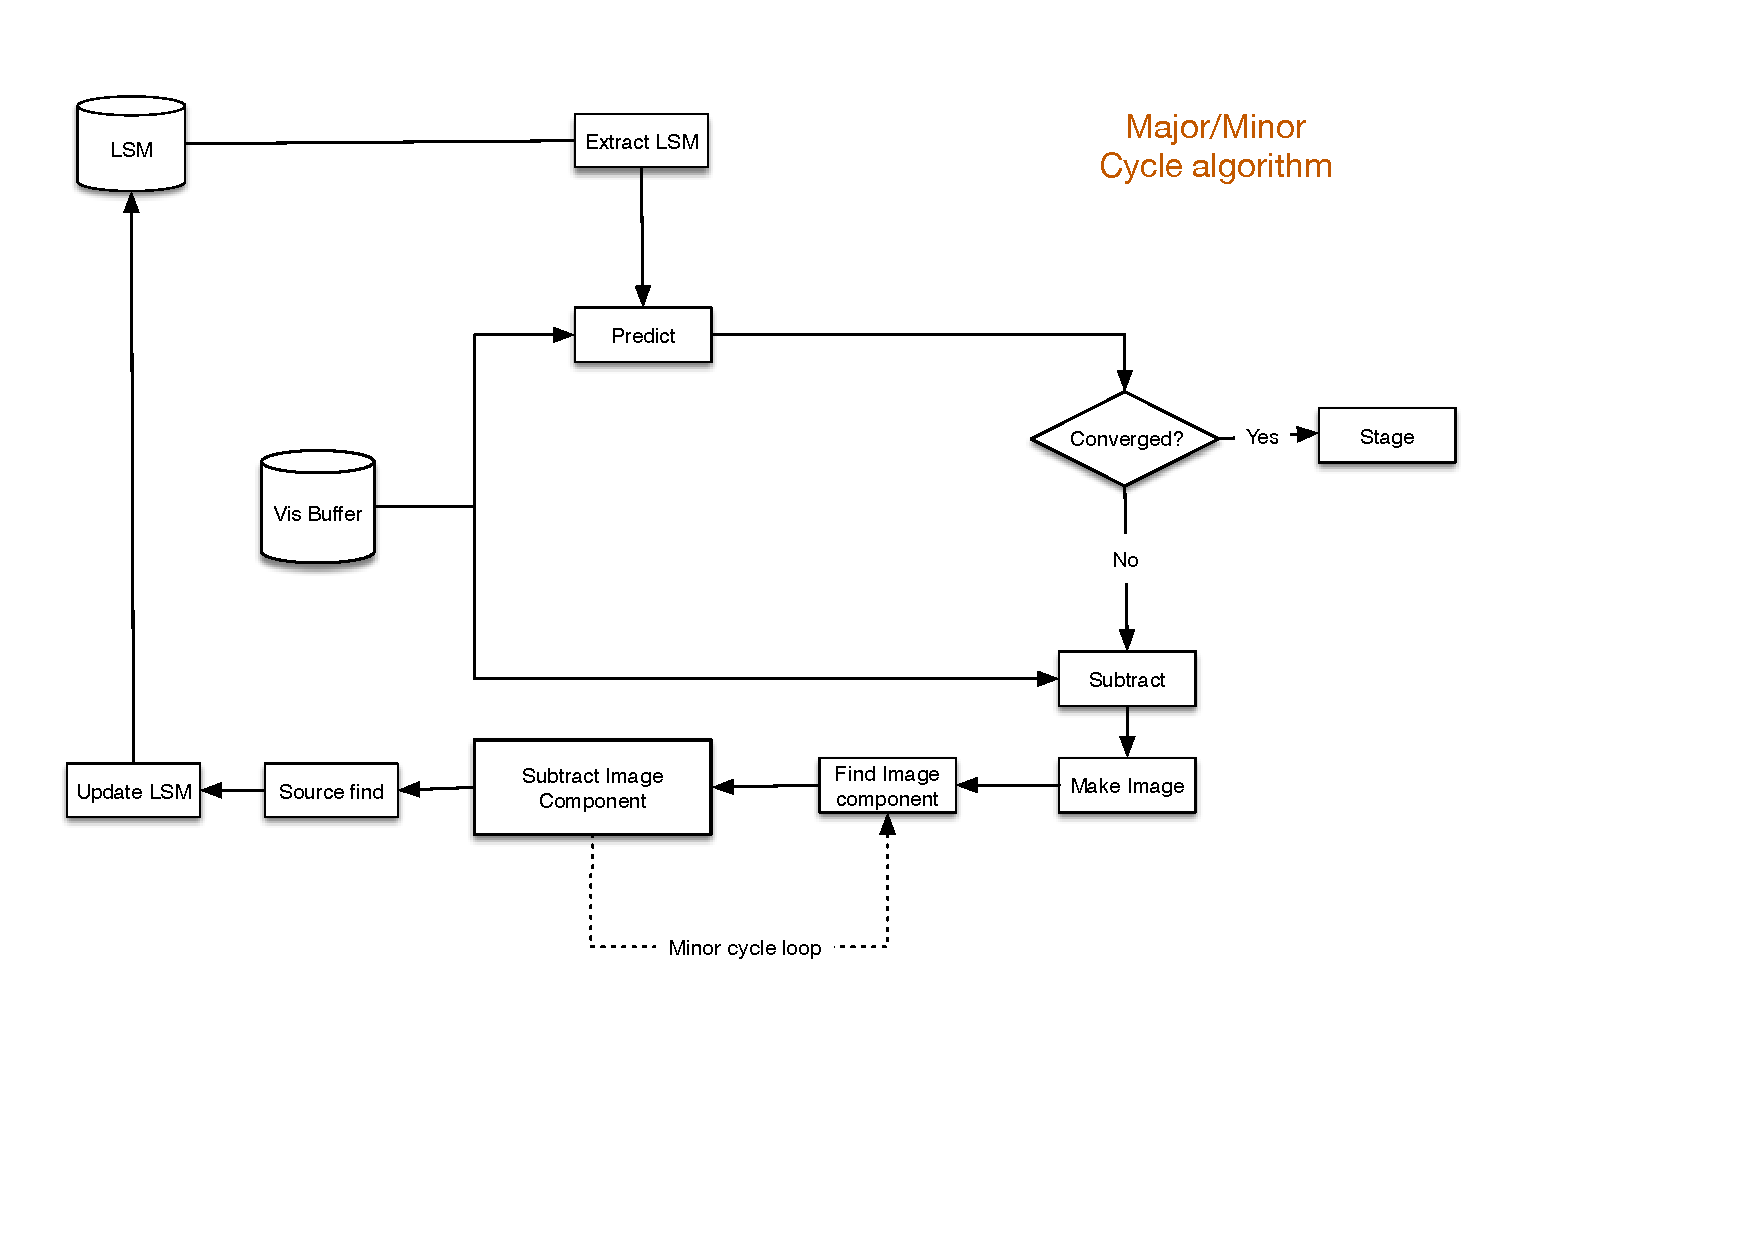
\includegraphics[width=\textwidth]{./MSMFS_MajorMinor.pdf}
  \caption{Structure of Major/Minor cycle algorithm}
  \label{fig:majorminor}
\end{figure}

The major cycle returns to the visibility data each iteration, whereas the minor cycle is entirely image-based.

MSMFS is relatively high in complexity because the usual CLEAN process is coupled over both scale (MSClean) and frequency or Taylor terms (MFS). The minor cycle must conduct a search in scale and Taylor term for each peak search. The major cycle requires calculation of the residual Taylor terms, which implies gridding and degridding all relevant frequency information. Memory use is high since a large number of images must be kept and updated as the iteration proceeds.


\begin{figure}[htb]
  \centering
  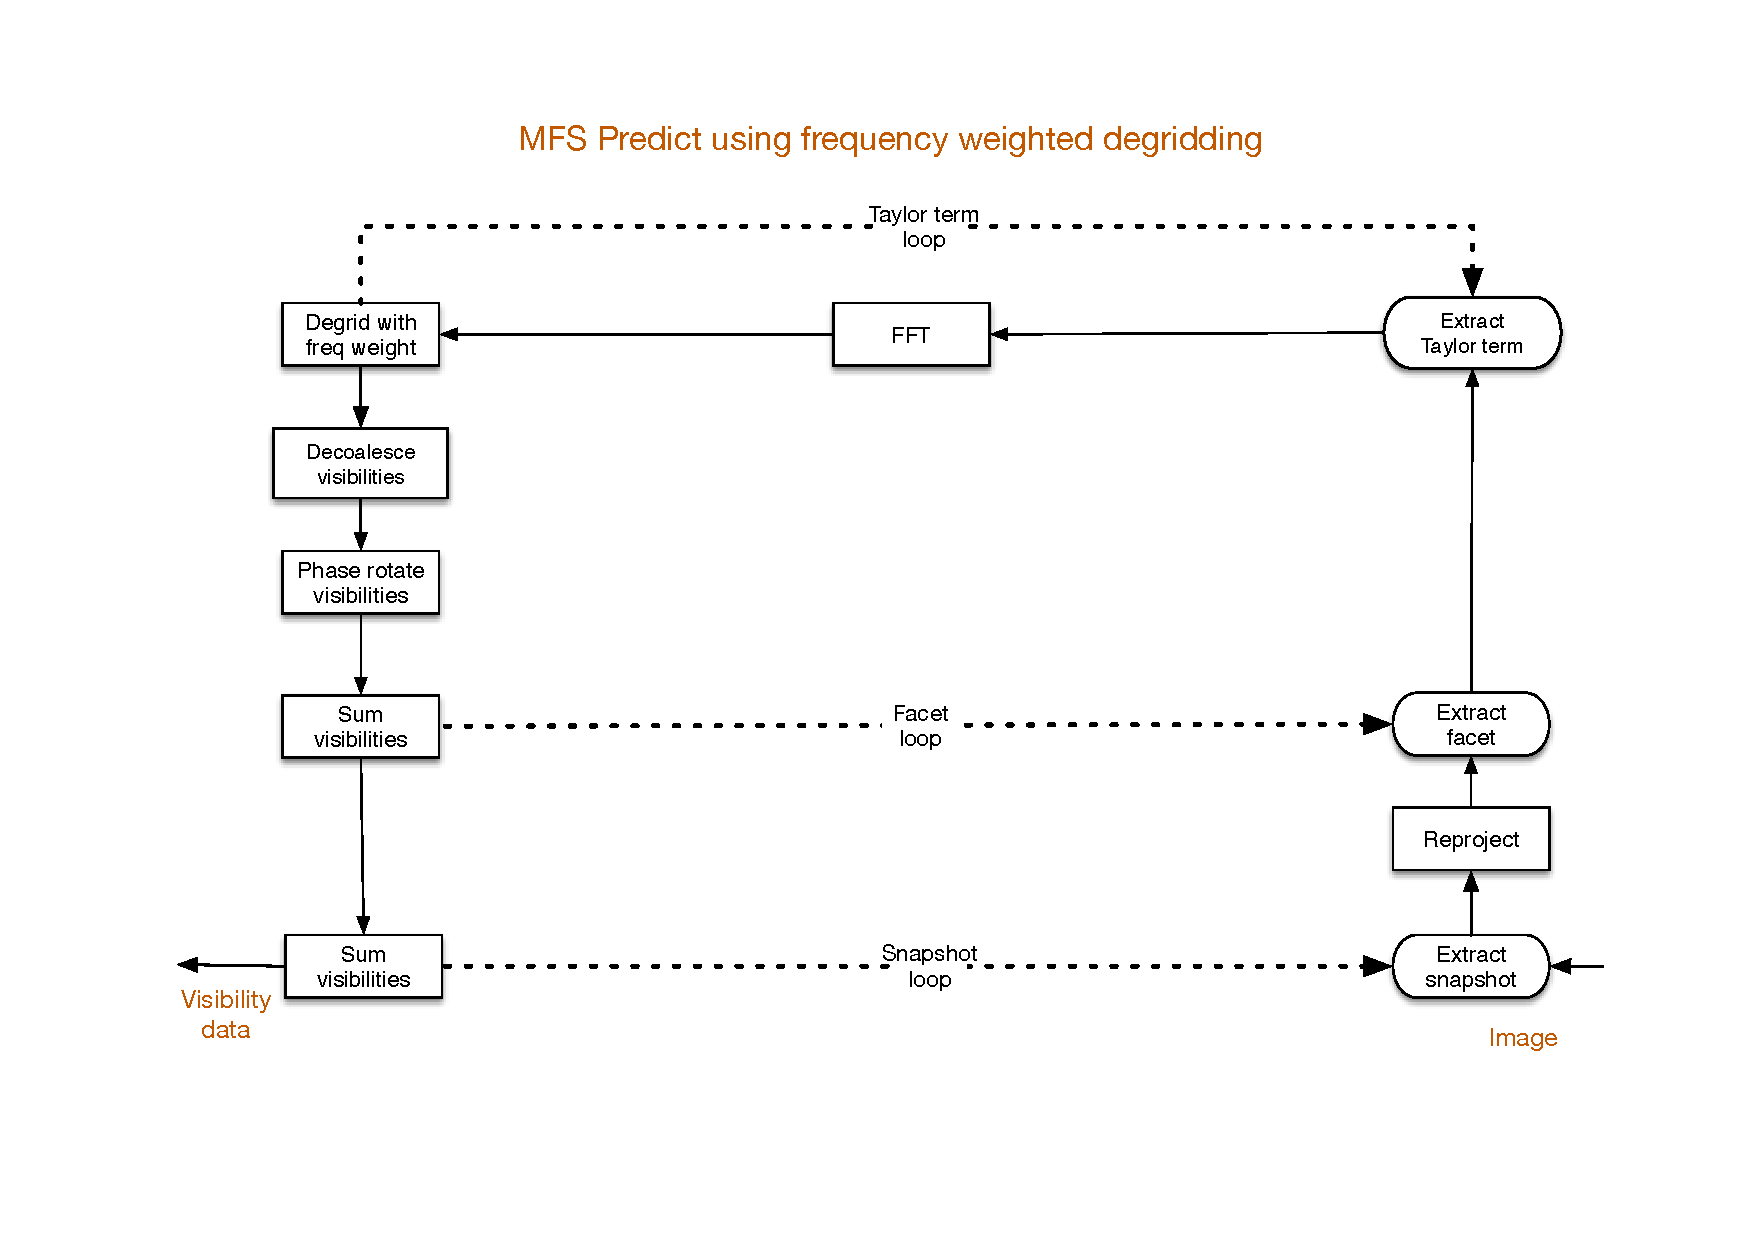
\includegraphics[width=\textwidth]{./MSMFS_Predict_UV.pdf}
  \caption{Structure of UV-weighting Predict, as used in ASKAPsoft. }
  \label{fig:predictuv}
\end{figure}

\begin{figure}[htb]
  \centering
  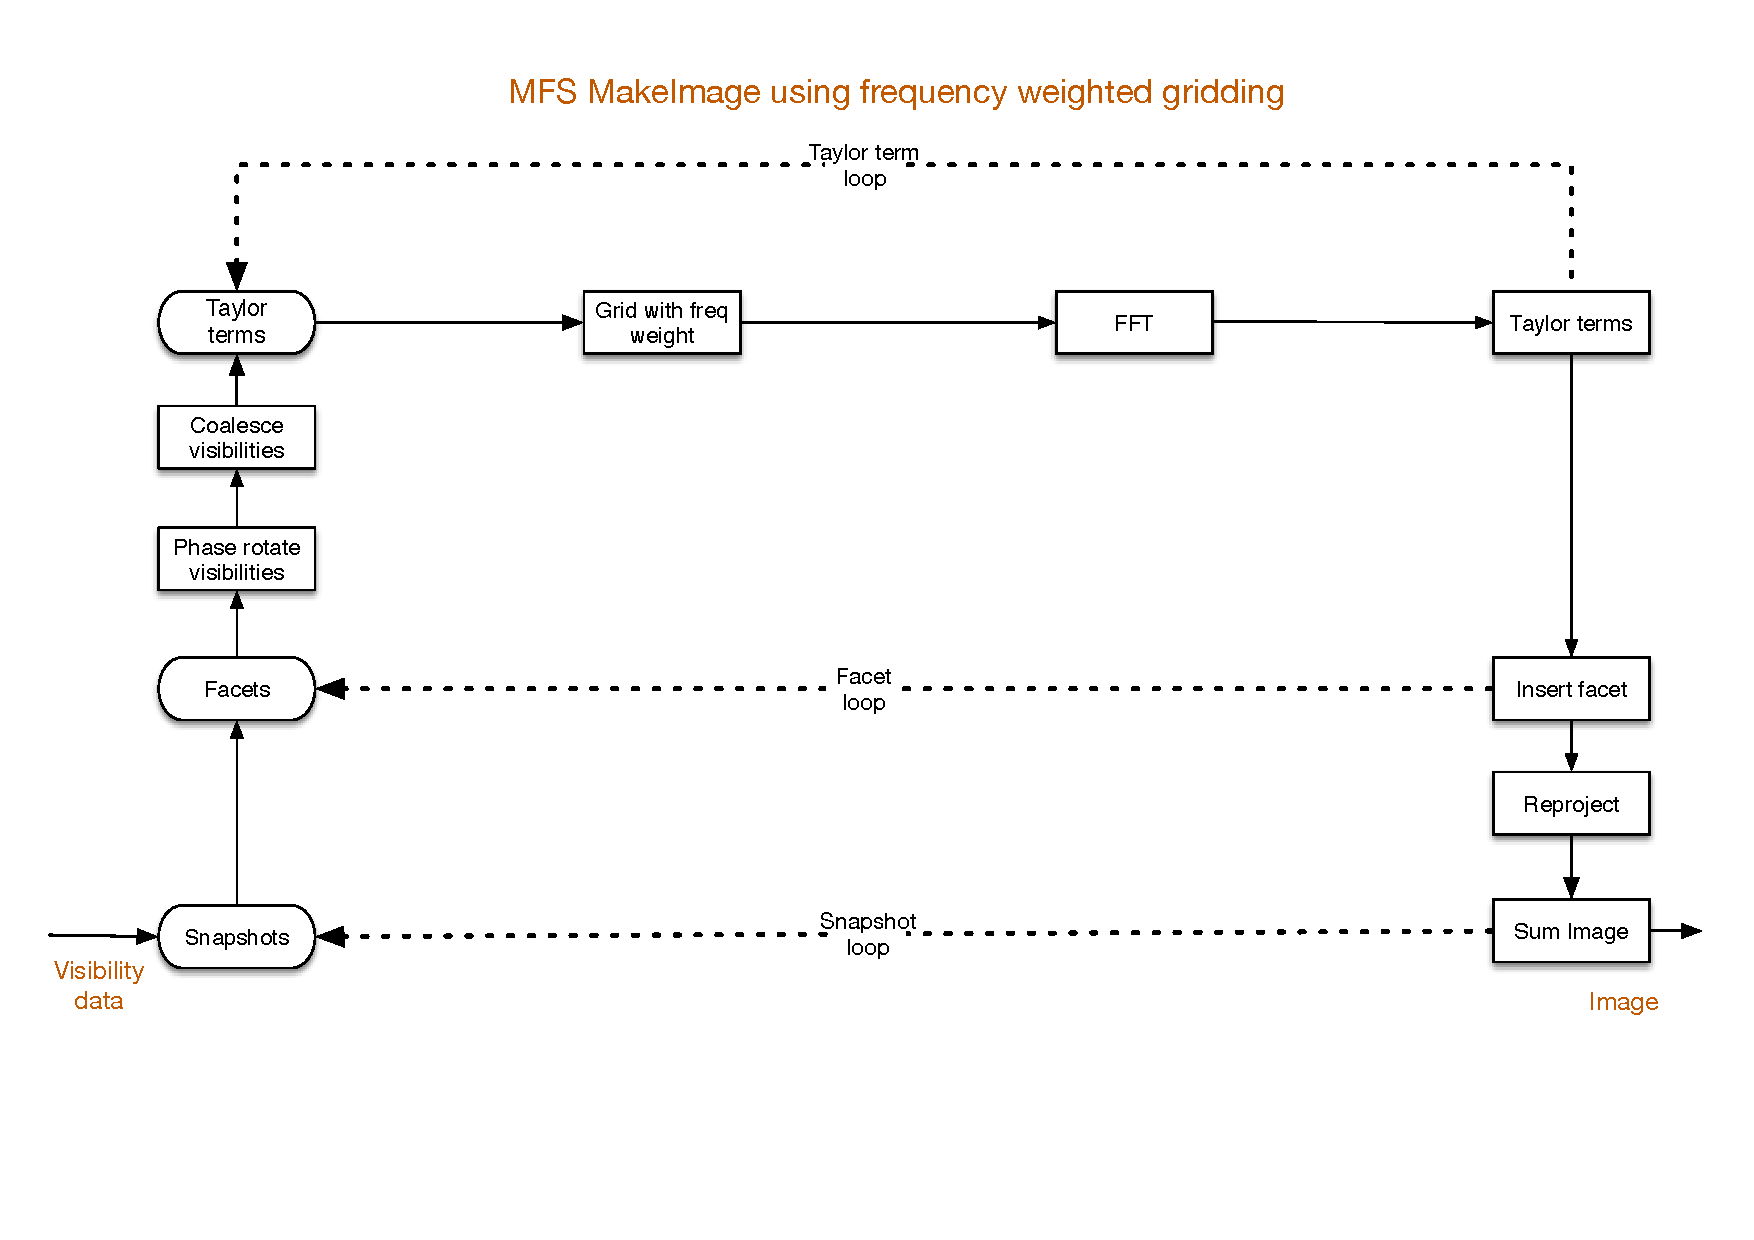
\includegraphics[width=\textwidth]{./MSMFS_MakeImage_UV.pdf}
  \caption{Structure of UV-weighting MakeImage, as used in ASKAPsoft. Note that the three loops (denoted by the rectangle with curved ends) can be permutated at will.}
  \label{fig:predictimage}
\end{figure}


\begin{figure}[htb]
  \centering
  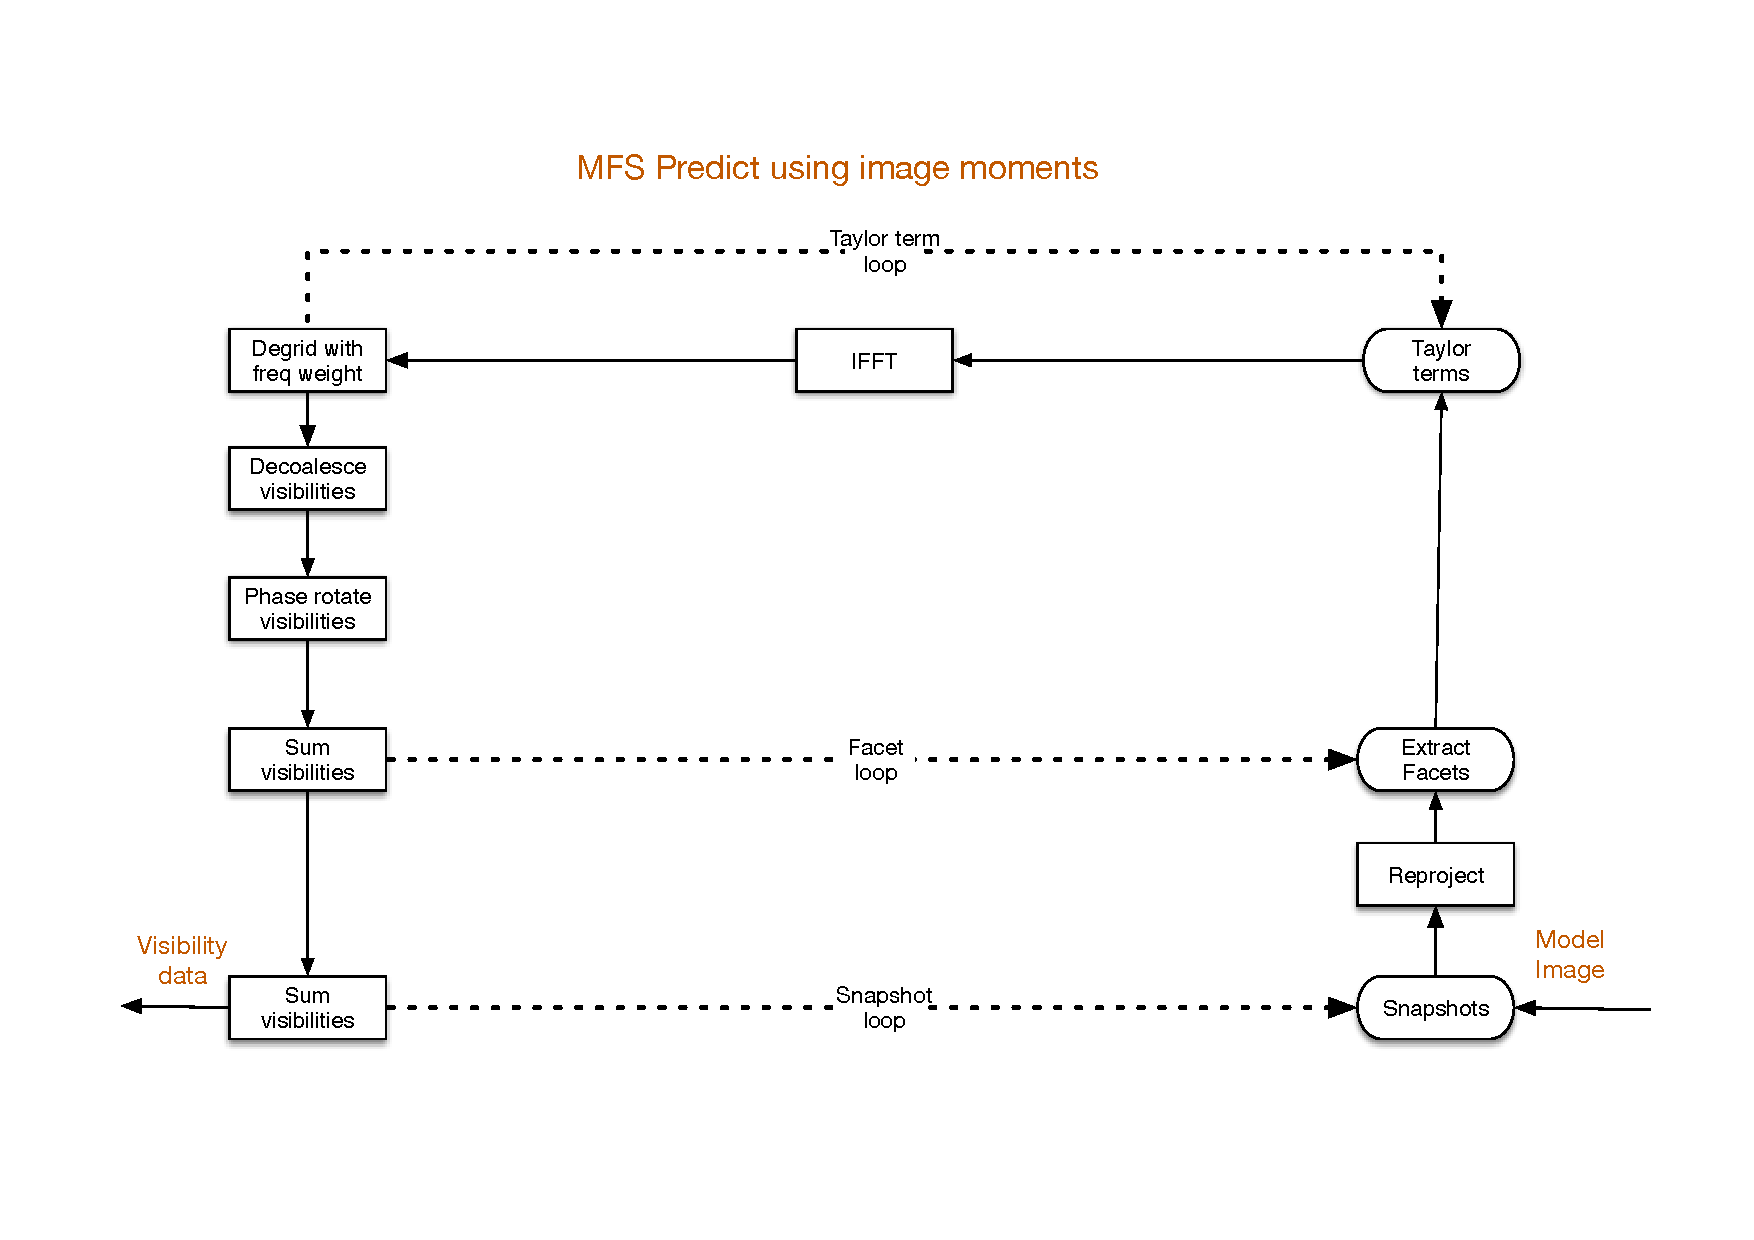
\includegraphics[width=\textwidth]{./MSMFS_Predict_Image.pdf}
  \caption{Structure of Image plane-weighting Predict, as used in CASA. Note that the three loops (denoted by the rectangle with curved ends) can be permutated at will.}
  \label{fig:makeimageuv}
\end{figure}


\begin{figure}[htb]
  \centering
  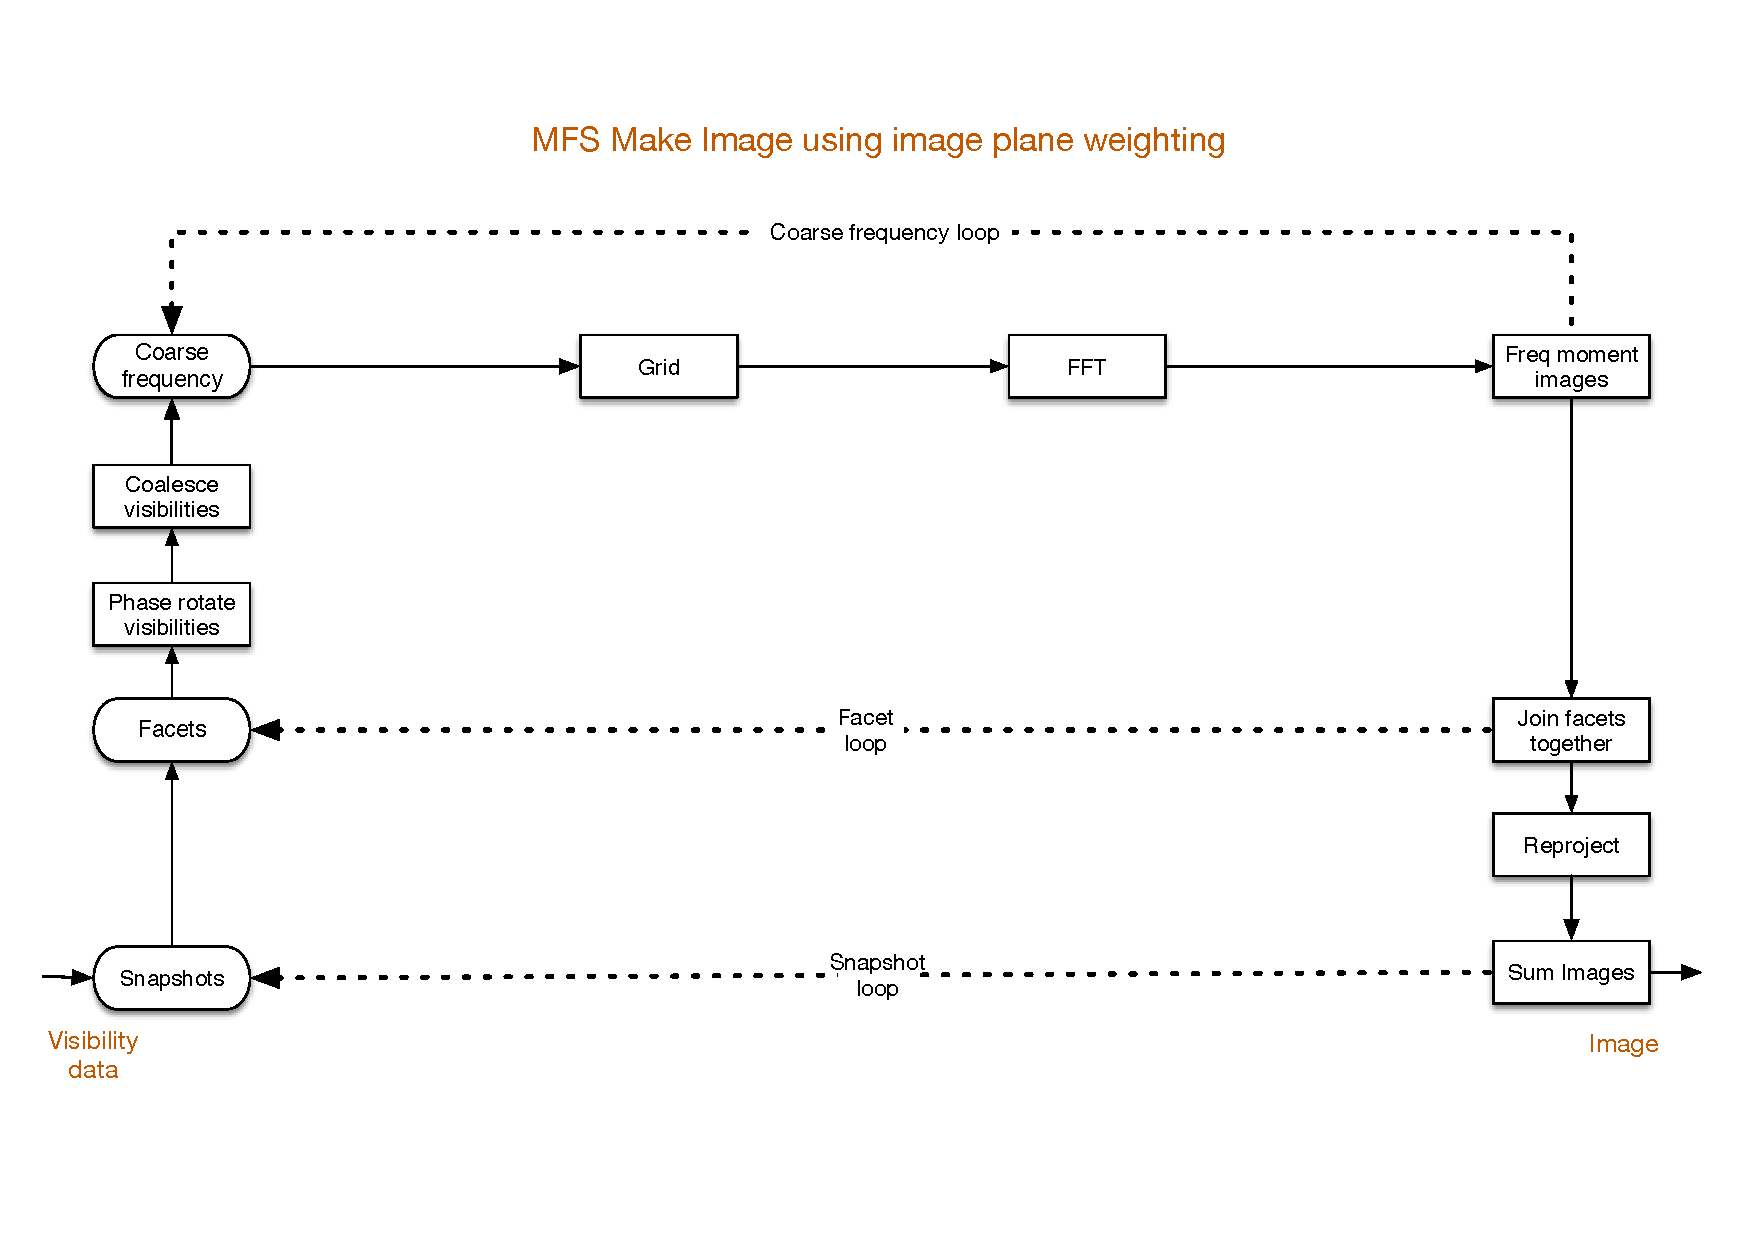
\includegraphics[width=\textwidth]{./MSMFS_MakeImage_Image.pdf}
  \caption{Structure of Image plane-weighting MakeImage, as used in CASA. Note that the three loops (denoted by the rectangle with curved ends) can be permuted at will.}
  \label{fig:makeimageimage}
\end{figure}

\clearpage
\section{Serial}
\label{sec:serial}

The serial algorithm is as shown in Algorithm \ref{alg:MSMFS_1}.

\begin{equation}
\vec{I}^{model} = \sum_{s=0}^{N_s-1}  \vec{I}^{shp}_{s} \star \vec{I}^{sky,\delta}_s
\label{Eq:ms_model}
\end{equation}

where $N_s$ is the number of spatial scales used to construct the image, and
$\vec{I}^{sky,\delta}_{s}$ represents a collection of $\delta$-functions that describe the locations
and integrated amplitudes of flux components of scale $s$ in the image. $\vec{I}^{shp}_s$ is a tapered truncated parabola of width proportional to $s$.
The symbol $\star$ denotes convolution. 

\begin{eqnarray}
\label{eqn:mf_model}
\vec{I}^{model}_{\nu} = \sum_{t=0}^{N_t-1} \wnt \vec{I}^{sky}_{t} ~~~\mathrm{where}~~~ \wnt&=&\dnuno^t 
\end{eqnarray}

where $N_t$ is the order of the Taylor series expansion, and 
the $I^m_t$ represent multi-scale Taylor coefficient images.

The image flux model at each frequency can be written as a linear sum of  
coefficient images at different spatial scales. 
\begin{equation}
\vec{I}^{model}_{\nu} = \sum_{t=0}^{N_t} \sum_{s=0}^{N_s} \wnt \left[ \vec{I}^{shp}_s \star \vec{I}^{sky}_\frac{s}{t}\right] ~~~~\mathrm{where}~~~\wnt = \dnuno^t 
\label{eqn:msmf_model}
\end{equation}

Here, $N_s$ is the number of discrete spatial scales used to represent the image and  
$N_t$ is the order of the series expansion of the spectrum. $\vec{I}^{sky}_\frac{s}{t}$ represents 
a collection of $\delta$-functions that describe the locations
and integrated amplitudes of flux components of scale $s$ in the image of the $t^{th}$ series 
coefficient. 

In words, the MSMFS algorithm decomposes the image into a set of blobs, using a greedy algorithm in which the peak (in scale space) is found by searching for the peak in the reference frequency residual images each convolved with scale. For bright pixels, the principal solution is calculated by applying the inverse Hessian of the PSF convolved with scale. For faint pixels, just the peak in the reference frequency image is used. 


\clearpage

\begin{algorithm}[t!]
\scriptsize
\label{alg:MSMFS_1}
%  \SetKwRepeat{Repeat}{Repeat}{Until}
%  \SetKwFor{ForEach}{ForEach}{Do}{End}
%\KwData{ $\vec{V}^{corr}_{\nu}, \vec{I}^{shp}_s~\forall~s\in\{0,N_s$-$1\}, ~ [\Sna]~ \forall \nu$ }
%\KwResult{ $\vec{I}^{psf}_{{sp}\atop{tq}},[{H^{peak}_s}], \vec{I}^m_{\nu_0}, \vec{I}^{\alpha}, \vec{I}^{\beta}$ }
  \KwData{calibrated visibilities : $\vec{V}^{corr}_{\nu}~~\forall \nu$}
  \KwData{$uv$-sampling function : $\Sna$}
  \KwData{image noise threshold and loop gain $\sigma_{thr}, g_s$}
  \KwData{scale basis functions : $\I^{shp}_s ~ \forall s\in\{0,N_s-1\}$}
  \KwResult{model coefficient images : $\I^{m}_{q}~ \forall q\in\{0,N_t-1\}$}
  \KwResult{spectral index and curvature : $\I^{m}_{\alpha},\I^{m}_{\beta}$}

  \vspace{0.5cm} 
%{Compute the dirty image $\vec{I}^{dirty}$ and psf $\vec{I}^{psf}$}\;
  \For{ $t \in \{0,N_t-1\}, q \in \{t,N_t-1\}$}
  {
        { Compute the spectral PSF } $\vec{I}^{psf}_{tq}$\;
        \For{ $s \in \{0,N_s-1\}, p \in \{s,N_s-1\}$}
	{
		{Compute the scale-spectral PSF} $\vec{I}^{psf}_{{sp}\atop{tq}} = \vec{I}^{shp}_s \star \vec{I}^{shp}_p \star \vec{I}^{psf}_{tq} $\;
	}
  }
  \For { $s \in \{0,N_s-1\}$}
  {
     Construct $[{H^{peak}_s}]$ from $mid(I^{psf}_{{s,s}\atop{t,q}})$ and compute $[{H^{peak}_s}^{-1}]$\;
  }
%%%%%%%%%%%%%%%%%%%%%%
%%%\vspace{0.5cm}
%%  \caption[MS-MFS CLEAN : Pre-Deconvolution Setup]
%%          {MS-MFS CLEAN : Pre-Deconvolution Setup}
%%\end{algorithm}
%%%\newpage
%%
%%\begin{algorithm}[H]
%%  \SetLine
%%  \linesnumbered
%%  \dontprintsemicolon
%%%%%%%%%%%%%%%%%%%%%%%  
%%\KwData{ $\vec{V}^{corr}_{\nu}, \vec{I}^{shp}_s, \vec{I}^{psf}_{{sp}\atop{tq}},[{H^{peak}_s}]~~~\forall~~s \in \{0,N_s-1\}, p \in \{s,N_s-1\}, \sigma_{thr}$ }
%%\KwResult{$I^{m}_{q}~ \forall q \in \{0,N_t-1\}$}
%%%%%%%%%%%%%%%%%%%%%  
  Initialize the model $\vec{I}^{m}_t$ for all $t \in \{0,N_t-1\}$ and compute $f_{sidelobe}$ \;
  \Repeat (\tcc*[f]{Major Cycle}) { Peak residual in $\vec{I}^{res}_0 < \sigma_{thr}$ }
  {
    \For{$t \in \{0,N_t$-$1\}$}
    {
      Compute the residual image $\vec{I}^{res}_t$ \tcc*[r]{Makeimage}
      \For{$s \in \{0,N_s$-$1\}$}
      {
	      Compute $\vec{I}^{res}_{{s},{t}} = \vec{I}^{shp}_s \star \vec{I}^{res}_t$
      }
    }
    Calculate $f_{limit}$ from $\vec{I}^{res}_{0,0}$\;
    \Repeat (\tcc*[f]{Minor Cycle}){ Peak residual in $\vec{I}^{res}_{0,0} < f_{limit} $ } 
    {
%     Compute $I^{m}_q~\forall q\in \{0.N_t-1\}$ and update $\vec{I}^{res}_{{s},{t}}~\forall s,t$ (Algorithm \vref{ALGO:MSMFS_2})\;
     \For{$s \in \{0,N_s$-$1\}$} 
     {
      \uIf{Peak of $\vec{I}^{res}_{s,0} > 10~\sigma_{thr} $}
      {
       \ForEach{pixel}
       {
          Construct $I^{rhs}_s$, an $N_t\times 1$ vector from $I^{res}_{s,t} ~~\forall ~ t \in \{0,N_t$-$1\}$\;
          Compute principal solution $I^{sol}_s = [{H^{peak}_s}^{-1}] I^{rhs}_s$\;
       }
       Choose $I^{sol} = max\{I^{sol}_{t=0},~\forall~s\in\{0,N_s$-$1\}\}$ \;
      }
      \Else
      {
       Find the location of the peak in $\vec{I}^{res}_{s,0},~\forall~s\in\{0,N_s$-$1\}$\;
       Construct $I^{rhs}_s$, from $I^{res}_{s,t}$ for the chosen $s$, at this location\;
       Compute $I^{sol} = [{H^{peak}_s}^{-1}] I^{rhs}_s$ at this location\;
      }
     }
       \For{$t \in \{0,N_t-1\}$}
       {
        Update the model image : $I^{m}_t = I^{m}_t + g_s ~ I^{shp}_{s_i} \star I^{sol}_t$ \;
        \For{$s \in \{0,N_s$-$1\}$}
	{
          Update the residual image : $I^{res}_{s,t} = I^{res}_{s,t} - g ~\sum_{p=0}^{N_s-1}\sum_{q=0}^{N_t-1}[I^{psf}_{{sp}\atop{tq}} \star I^{sol}_q]$\;
	}
       }
    }
   Compute model visibilities $V^{m}_{\nu}$ from  $I^{m}_t~\forall t\in \{0.N_t-1\}$\tcc*[r]{Predict} 
   Compute a new residual image $I^{res}$ from residual visibilities $V^{corr}_{\nu}-V^{m}_{\nu}$ \tcc*[r]{Makeimage}
}
Calculate $\vec{I}^m_{\nu_0}, \vec{I}^{\alpha}, \vec{I}^{\beta}$ from $I^{m}_t~\forall t\in \{0.N_t-1\}$ and restore the results \;
If required, remove average primary beam : $\vec{I}^{new}_{\nu_0}=\vec{I}^m_{\nu_0}/\vec{\Pb}_{\nu_0}, \vec{I}^{new}_{\alpha}=\vec{I}^m_{\alpha}-\vec{\Pb}_{\alpha}, \vec{I}^{new}_{\beta}=\vec{I}^m_{\beta}-\vec{\Pb}_{\beta}$\;
\vspace{0.5cm}

  \caption[MS-MFS Algorithm]
          {MS-MFS Algorithm : }
\end{algorithm}

Notes:
\begin{description}
\item[Line 13]	
\end{description}


\clearpage
\section{Partitioning}
\label{sec:partitioning}

The SDP pipeline framework [RD:??], allows partitioning across multiple axes. In this case, the natural partitions are:

\begin{description}
\item[Frequency]
\item[Time]
\item[Facet]
\item[Scales]	
\end{description}


\clearpage
\section{A projection}
\label{sec:minor}

\clearpage
\section{Wide-band behaviour}
\label{sec:wideband}

\begin{itemize}
\item Does naive broadband work?
\item Bhatnagar et al WB algorithm	
\end{itemize}


\clearpage
\section{Modelling MSMFS in the SDP Performance Manager}
\label{sec:modelling}

\clearpage
\section{Resource usage}
\label{sec:resource}


% \label{section:main}



% Add the bibliography
\clearpage \addcontentsline{toc}{section}{References}
\bibliography{your_bibfile}%



\end{document}

%%% Local Variables: 
%%% mode: latex
%%% TeX-master: t
%%% End: 
